\documentclass[1p]{elsarticle_modified}
%\bibliographystyle{elsarticle-num}

%\usepackage[colorlinks]{hyperref}
%\usepackage{abbrmath_seonhwa} %\Abb, \Ascr, \Acal ,\Abf, \Afrak
\usepackage{amsfonts}
\usepackage{amssymb}
\usepackage{amsmath}
\usepackage{amsthm}
\usepackage{scalefnt}
\usepackage{amsbsy}
\usepackage{kotex}
\usepackage{caption}
\usepackage{subfig}
\usepackage{color}
\usepackage{graphicx}
\usepackage{xcolor} %% white, black, red, green, blue, cyan, magenta, yellow
\usepackage{float}
\usepackage{setspace}
\usepackage{hyperref}

\usepackage{tikz}
\usetikzlibrary{arrows}

\usepackage{multirow}
\usepackage{array} % fixed length table
\usepackage{hhline}

%%%%%%%%%%%%%%%%%%%%%
\makeatletter
\renewcommand*\env@matrix[1][\arraystretch]{%
	\edef\arraystretch{#1}%
	\hskip -\arraycolsep
	\let\@ifnextchar\new@ifnextchar
	\array{*\c@MaxMatrixCols c}}
\makeatother %https://tex.stackexchange.com/questions/14071/how-can-i-increase-the-line-spacing-in-a-matrix
%%%%%%%%%%%%%%%

\usepackage[normalem]{ulem}

\newcommand{\msout}[1]{\ifmmode\text{\sout{\ensuremath{#1}}}\else\sout{#1}\fi}
%SOURCE: \msout is \stkout macro in https://tex.stackexchange.com/questions/20609/strikeout-in-math-mode

\newcommand{\cancel}[1]{
	\ifmmode
	{\color{red}\msout{#1}}
	\else
	{\color{red}\sout{#1}}
	\fi
}

\newcommand{\add}[1]{
	{\color{blue}\uwave{#1}}
}

\newcommand{\replace}[2]{
	\ifmmode
	{\color{red}\msout{#1}}{\color{blue}\uwave{#2}}
	\else
	{\color{red}\sout{#1}}{\color{blue}\uwave{#2}}
	\fi
}

\newcommand{\Sol}{\mathcal{S}} %segment
\newcommand{\D}{D} %diagram
\newcommand{\A}{\mathcal{A}} %arc


%%%%%%%%%%%%%%%%%%%%%%%%%%%%%5 test

\def\sl{\operatorname{\textup{SL}}(2,\Cbb)}
\def\psl{\operatorname{\textup{PSL}}(2,\Cbb)}
\def\quan{\mkern 1mu \triangleright \mkern 1mu}

\theoremstyle{definition}
\newtheorem{thm}{Theorem}[section]
\newtheorem{prop}[thm]{Proposition}
\newtheorem{lem}[thm]{Lemma}
\newtheorem{ques}[thm]{Question}
\newtheorem{cor}[thm]{Corollary}
\newtheorem{defn}[thm]{Definition}
\newtheorem{exam}[thm]{Example}
\newtheorem{rmk}[thm]{Remark}
\newtheorem{alg}[thm]{Algorithm}

\newcommand{\I}{\sqrt{-1}}
\begin{document}

%\begin{frontmatter}
%
%\title{Boundary parabolic representations of knots up to 8 crossings}
%
%%% Group authors per affiliation:
%\author{Yunhi Cho} 
%\address{Department of Mathematics, University of Seoul, Seoul, Korea}
%\ead{yhcho@uos.ac.kr}
%
%
%\author{Seonhwa Kim} %\fnref{s_kim}}
%\address{Center for Geometry and Physics, Institute for Basic Science, Pohang, 37673, Korea}
%\ead{ryeona17@ibs.re.kr}
%
%\author{Hyuk Kim}
%\address{Department of Mathematical Sciences, Seoul National University, Seoul 08826, Korea}
%\ead{hyukkim@snu.ac.kr}
%
%\author{Seokbeom Yoon}
%\address{Department of Mathematical Sciences, Seoul National University, Seoul, 08826,  Korea}
%\ead{sbyoon15@snu.ac.kr}
%
%\begin{abstract}
%We find all boundary parabolic representation of knots up to 8 crossings.
%
%\end{abstract}
%\begin{keyword}
%    \MSC[2010] 57M25 
%\end{keyword}
%
%\end{frontmatter}

%\linenumbers
%\tableofcontents
%
\newcommand\colored[1]{\textcolor{white}{\rule[-0.35ex]{0.8em}{1.4ex}}\kern-0.8em\color{red} #1}%
%\newcommand\colored[1]{\textcolor{white}{ #1}\kern-2.17ex	\textcolor{white}{ #1}\kern-1.81ex	\textcolor{white}{ #1}\kern-2.15ex\color{red}#1	}

{\Large $\underline{12a_{0339}~(K12a_{0339})}$}

\setlength{\tabcolsep}{10pt}
\renewcommand{\arraystretch}{1.6}
\vspace{1cm}\begin{tabular}{m{100pt}>{\centering\arraybackslash}m{274pt}}
\multirow{5}{120pt}{
	\centering
	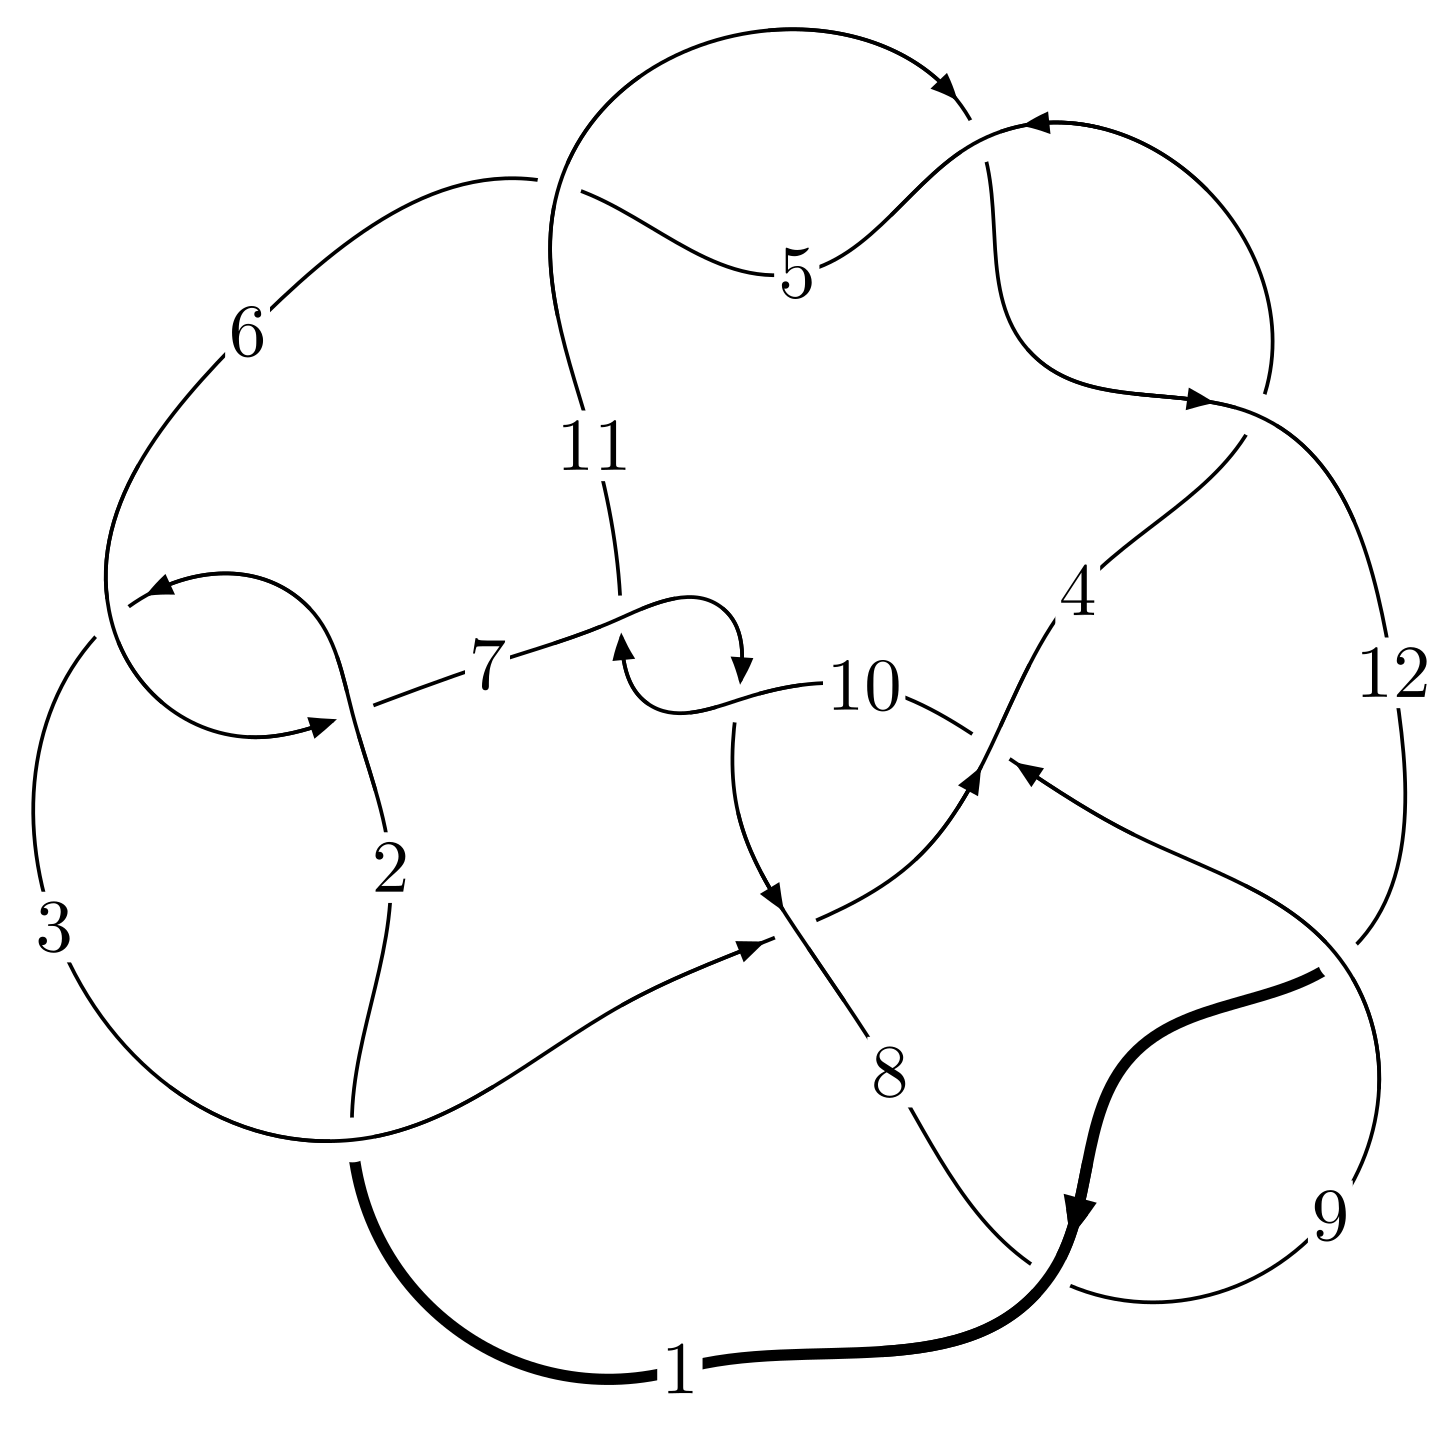
\includegraphics[width=112pt]{../../../GIT/diagram.site/Diagrams/png/1140_12a_0339.png}\\
\ \ \ A knot diagram\footnotemark}&
\allowdisplaybreaks
\textbf{Linearized knot diagam} \\
\cline{2-2}
 &
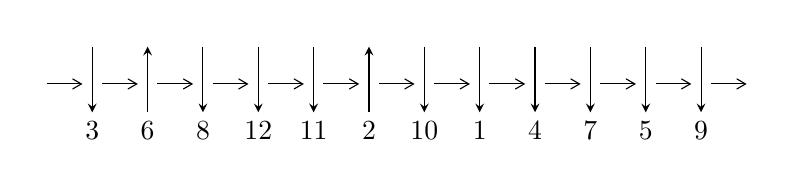
\begin{tikzpicture}[x=20pt, y=17pt]
	% nodes
	\node (C0) at (0, 0) {};
	\node (C1) at (1, 0) {};
	\node (C1U) at (1, +1) {};
	\node (C1D) at (1, -1) {3};

	\node (C2) at (2, 0) {};
	\node (C2U) at (2, +1) {};
	\node (C2D) at (2, -1) {6};

	\node (C3) at (3, 0) {};
	\node (C3U) at (3, +1) {};
	\node (C3D) at (3, -1) {8};

	\node (C4) at (4, 0) {};
	\node (C4U) at (4, +1) {};
	\node (C4D) at (4, -1) {12};

	\node (C5) at (5, 0) {};
	\node (C5U) at (5, +1) {};
	\node (C5D) at (5, -1) {11};

	\node (C6) at (6, 0) {};
	\node (C6U) at (6, +1) {};
	\node (C6D) at (6, -1) {2};

	\node (C7) at (7, 0) {};
	\node (C7U) at (7, +1) {};
	\node (C7D) at (7, -1) {10};

	\node (C8) at (8, 0) {};
	\node (C8U) at (8, +1) {};
	\node (C8D) at (8, -1) {1};

	\node (C9) at (9, 0) {};
	\node (C9U) at (9, +1) {};
	\node (C9D) at (9, -1) {4};

	\node (C10) at (10, 0) {};
	\node (C10U) at (10, +1) {};
	\node (C10D) at (10, -1) {7};

	\node (C11) at (11, 0) {};
	\node (C11U) at (11, +1) {};
	\node (C11D) at (11, -1) {5};

	\node (C12) at (12, 0) {};
	\node (C12U) at (12, +1) {};
	\node (C12D) at (12, -1) {9};
	\node (C13) at (13, 0) {};

	% arrows
	\draw[->,>={angle 60}]
	(C0) edge (C1) (C1) edge (C2) (C2) edge (C3) (C3) edge (C4) (C4) edge (C5) (C5) edge (C6) (C6) edge (C7) (C7) edge (C8) (C8) edge (C9) (C9) edge (C10) (C10) edge (C11) (C11) edge (C12) (C12) edge (C13) ;	\draw[->,>=stealth]
	(C1U) edge (C1D) (C2D) edge (C2U) (C3U) edge (C3D) (C4U) edge (C4D) (C5U) edge (C5D) (C6D) edge (C6U) (C7U) edge (C7D) (C8U) edge (C8D) (C9U) edge (C9D) (C10U) edge (C10D) (C11U) edge (C11D) (C12U) edge (C12D) ;
	\end{tikzpicture} \\
\hhline{~~} \\& 
\textbf{Solving Sequence} \\ \cline{2-2} 
 &
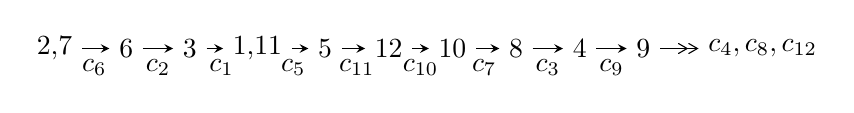
\begin{tikzpicture}[x=23pt, y=7pt]
	% node
	\node (A0) at (-1/8, 0) {2,7};
	\node (A1) at (1, 0) {6};
	\node (A2) at (2, 0) {3};
	\node (A3) at (49/16, 0) {1,11};
	\node (A4) at (33/8, 0) {5};
	\node (A5) at (41/8, 0) {12};
	\node (A6) at (49/8, 0) {10};
	\node (A7) at (57/8, 0) {8};
	\node (A8) at (65/8, 0) {4};
	\node (A9) at (73/8, 0) {9};
	\node (C1) at (1/2, -1) {$c_{6}$};
	\node (C2) at (3/2, -1) {$c_{2}$};
	\node (C3) at (5/2, -1) {$c_{1}$};
	\node (C4) at (29/8, -1) {$c_{5}$};
	\node (C5) at (37/8, -1) {$c_{11}$};
	\node (C6) at (45/8, -1) {$c_{10}$};
	\node (C7) at (53/8, -1) {$c_{7}$};
	\node (C8) at (61/8, -1) {$c_{3}$};
	\node (C9) at (69/8, -1) {$c_{9}$};
	\node (A10) at (11, 0) {$c_{4},c_{8},c_{12}$};

	% edge
	\draw[->,>=stealth]	
	(A0) edge (A1) (A1) edge (A2) (A2) edge (A3) (A3) edge (A4) (A4) edge (A5) (A5) edge (A6) (A6) edge (A7) (A7) edge (A8) (A8) edge (A9) ;
	\draw[->>,>={angle 60}]	
	(A9) edge (A10);
\end{tikzpicture} \\ 

\end{tabular} \\

\footnotetext{
The image of knot diagram is generated by the software ``\textbf{Draw programme}" developed by Andrew Bartholomew(\url{http://www.layer8.co.uk/maths/draw/index.htm\#Running-draw}), where we modified some parts for our purpose(\url{https://github.com/CATsTAILs/LinksPainter}).
}\phantom \\ \newline 
\centering \textbf{Ideals for irreducible components\footnotemark of $X_{\text{par}}$} 
 
\begin{align*}
I^u_{1}&=\langle 
-8.07878\times10^{237} u^{106}-5.69593\times10^{238} u^{105}+\cdots+1.02698\times10^{240} b-4.14748\times10^{240},\\
\phantom{I^u_{1}}&\phantom{= \langle  }-1.16910\times10^{241} u^{106}-1.12816\times10^{239} u^{105}+\cdots+1.95127\times10^{241} a+9.47218\times10^{241},\\
\phantom{I^u_{1}}&\phantom{= \langle  }u^{107}+18 u^{105}+\cdots-24 u+19\rangle \\
I^u_{2}&=\langle 
2130709 u^{29}+9442748 u^{28}+\cdots+3960308 b-4255385,\\
\phantom{I^u_{2}}&\phantom{= \langle  }29240837 u^{29}+79392300 u^{28}+\cdots+3960308 a+20834703,\;u^{30}+3 u^{29}+\cdots+3 u+1\rangle \\
\\
\end{align*}
\raggedright * 2 irreducible components of $\dim_{\mathbb{C}}=0$, with total 137 representations.\\
\footnotetext{All coefficients of polynomials are rational numbers. But the coefficients are sometimes approximated in decimal forms when there is not enough margin.}
\newpage
\renewcommand{\arraystretch}{1}
\centering \section*{I. $I^u_{1}= \langle -8.08\times10^{237} u^{106}-5.70\times10^{238} u^{105}+\cdots+1.03\times10^{240} b-4.15\times10^{240},\;-1.17\times10^{241} u^{106}-1.13\times10^{239} u^{105}+\cdots+1.95\times10^{241} a+9.47\times10^{241},\;u^{107}+18 u^{105}+\cdots-24 u+19 \rangle$}
\flushleft \textbf{(i) Arc colorings}\\
\begin{tabular}{m{7pt} m{180pt} m{7pt} m{180pt} }
\flushright $a_{2}=$&$\begin{pmatrix}0\\u\end{pmatrix}$ \\
\flushright $a_{7}=$&$\begin{pmatrix}1\\0\end{pmatrix}$ \\
\flushright $a_{6}=$&$\begin{pmatrix}1\\u^2\end{pmatrix}$ \\
\flushright $a_{3}=$&$\begin{pmatrix}u\\u^3+u\end{pmatrix}$ \\
\flushright $a_{1}=$&$\begin{pmatrix}u^3\\u^5+u^3+u\end{pmatrix}$ \\
\flushright $a_{11}=$&$\begin{pmatrix}0.599149 u^{106}+0.00578167 u^{105}+\cdots+103.443 u-4.85437\\0.00786652 u^{106}+0.0554628 u^{105}+\cdots+0.975711 u+4.03851\end{pmatrix}$ \\
\flushright $a_{5}=$&$\begin{pmatrix}0.348441 u^{106}+0.156526 u^{105}+\cdots+29.4128 u+21.6924\\-0.124729 u^{106}+0.120186 u^{105}+\cdots-23.9076 u+11.2074\end{pmatrix}$ \\
\flushright $a_{12}=$&$\begin{pmatrix}0.639779 u^{106}+0.0436662 u^{105}+\cdots+4.19949 u+9.11629\\-0.386630 u^{106}-0.0480225 u^{105}+\cdots-21.3738 u-3.87734\end{pmatrix}$ \\
\flushright $a_{10}=$&$\begin{pmatrix}0.607015 u^{106}+0.0612445 u^{105}+\cdots+104.419 u-0.815863\\0.00786652 u^{106}+0.0554628 u^{105}+\cdots+0.975711 u+4.03851\end{pmatrix}$ \\
\flushright $a_{8}=$&$\begin{pmatrix}-0.0125601 u^{106}-0.317357 u^{105}+\cdots+10.5566 u-28.4105\\0.0872593 u^{106}-0.0226541 u^{105}+\cdots+18.7313 u-5.60808\end{pmatrix}$ \\
\flushright $a_{4}=$&$\begin{pmatrix}0.871461 u^{106}+0.0699016 u^{105}+\cdots+16.2492 u+13.5251\\0.0417297 u^{106}-0.0636946 u^{105}+\cdots+15.8940 u-0.754748\end{pmatrix}$ \\
\flushright $a_{9}=$&$\begin{pmatrix}-0.0195297 u^{106}-0.335972 u^{105}+\cdots+11.9948 u-29.6475\\0.0902868 u^{106}+0.0286647 u^{105}+\cdots+14.7293 u-1.68637\end{pmatrix}$\\&\end{tabular}
\flushleft \textbf{(ii) Obstruction class $= -1$}\\~\\
\flushleft \textbf{(iii) Cusp Shapes $= 1.29735 u^{106}+0.145247 u^{105}+\cdots+65.0366 u+28.0789$}\\~\\
\newpage\renewcommand{\arraystretch}{1}
\flushleft \textbf{(iv) u-Polynomials at the component}\newline \\
\begin{tabular}{m{50pt}|m{274pt}}
Crossings & \hspace{64pt}u-Polynomials at each crossing \\
\hline $$\begin{aligned}c_{1}\end{aligned}$$&$\begin{aligned}
&u^{107}+36 u^{106}+\cdots-16866 u-361
\end{aligned}$\\
\hline $$\begin{aligned}c_{2},c_{6}\end{aligned}$$&$\begin{aligned}
&u^{107}+18 u^{105}+\cdots-24 u+19
\end{aligned}$\\
\hline $$\begin{aligned}c_{3}\end{aligned}$$&$\begin{aligned}
&u^{107}- u^{106}+\cdots+875682 u+270676
\end{aligned}$\\
\hline $$\begin{aligned}c_{4},c_{5},c_{11}\end{aligned}$$&$\begin{aligned}
&u^{107}+u^{106}+\cdots-3823 u+653
\end{aligned}$\\
\hline $$\begin{aligned}c_{7},c_{10}\end{aligned}$$&$\begin{aligned}
&u^{107}-5 u^{106}+\cdots-1215 u+43
\end{aligned}$\\
\hline $$\begin{aligned}c_{8},c_{12}\end{aligned}$$&$\begin{aligned}
&u^{107}+3 u^{106}+\cdots+90 u+68
\end{aligned}$\\
\hline $$\begin{aligned}c_{9}\end{aligned}$$&$\begin{aligned}
&u^{107}+u^{106}+\cdots+33976041 u+5654997
\end{aligned}$\\
\hline
\end{tabular}\\~\\
\newpage\renewcommand{\arraystretch}{1}
\flushleft \textbf{(v) Riley Polynomials at the component}\newline \\
\begin{tabular}{m{50pt}|m{274pt}}
Crossings & \hspace{64pt}Riley Polynomials at each crossing \\
\hline $$\begin{aligned}c_{1}\end{aligned}$$&$\begin{aligned}
&y^{107}+84 y^{106}+\cdots+71806242 y-130321
\end{aligned}$\\
\hline $$\begin{aligned}c_{2},c_{6}\end{aligned}$$&$\begin{aligned}
&y^{107}+36 y^{106}+\cdots-16866 y-361
\end{aligned}$\\
\hline $$\begin{aligned}c_{3}\end{aligned}$$&$\begin{aligned}
&y^{107}+45 y^{106}+\cdots-2480148075396 y-73265496976
\end{aligned}$\\
\hline $$\begin{aligned}c_{4},c_{5},c_{11}\end{aligned}$$&$\begin{aligned}
&y^{107}+123 y^{106}+\cdots-13417961 y-426409
\end{aligned}$\\
\hline $$\begin{aligned}c_{7},c_{10}\end{aligned}$$&$\begin{aligned}
&y^{107}+87 y^{106}+\cdots+85175 y-1849
\end{aligned}$\\
\hline $$\begin{aligned}c_{8},c_{12}\end{aligned}$$&$\begin{aligned}
&y^{107}+85 y^{106}+\cdots-46708 y-4624
\end{aligned}$\\
\hline $$\begin{aligned}c_{9}\end{aligned}$$&$\begin{aligned}
&y^{107}+57 y^{106}+\cdots-1085652345824199 y-31978991070009
\end{aligned}$\\
\hline
\end{tabular}\\~\\
\newpage\flushleft \textbf{(vi) Complex Volumes and Cusp Shapes}
$$\begin{array}{c|c|c}  
\text{Solutions to }I^u_{1}& \I (\text{vol} + \sqrt{-1}CS) & \text{Cusp shape}\\
 \hline 
\begin{aligned}
u &= \phantom{-}0.062374 + 1.007540 I \\
a &= -0.796736 + 1.058810 I \\
b &= \phantom{-}0.457334 - 0.922934 I\end{aligned}
 & -1.40043 + 2.59202 I & \phantom{-0.000000 } 0 \\ \hline\begin{aligned}
u &= \phantom{-}0.062374 - 1.007540 I \\
a &= -0.796736 - 1.058810 I \\
b &= \phantom{-}0.457334 + 0.922934 I\end{aligned}
 & -1.40043 - 2.59202 I & \phantom{-0.000000 } 0 \\ \hline\begin{aligned}
u &= -0.539561 + 0.857006 I \\
a &= -0.873556 + 1.018200 I \\
b &= \phantom{-}1.183120 - 0.066566 I\end{aligned}
 & -1.44165 - 2.15650 I & \phantom{-0.000000 } 0 \\ \hline\begin{aligned}
u &= -0.539561 - 0.857006 I \\
a &= -0.873556 - 1.018200 I \\
b &= \phantom{-}1.183120 + 0.066566 I\end{aligned}
 & -1.44165 + 2.15650 I & \phantom{-0.000000 } 0 \\ \hline\begin{aligned}
u &= \phantom{-}0.025107 + 1.017280 I \\
a &= \phantom{-}1.248120 - 0.139495 I \\
b &= -0.634688 - 0.196469 I\end{aligned}
 & -0.98241 + 1.99627 I & \phantom{-0.000000 } 0 \\ \hline\begin{aligned}
u &= \phantom{-}0.025107 - 1.017280 I \\
a &= \phantom{-}1.248120 + 0.139495 I \\
b &= -0.634688 + 0.196469 I\end{aligned}
 & -0.98241 - 1.99627 I & \phantom{-0.000000 } 0 \\ \hline\begin{aligned}
u &= -0.023639 + 0.981626 I \\
a &= \phantom{-}0.21172 + 2.86791 I \\
b &= -0.262160 - 1.223870 I\end{aligned}
 & \phantom{-}9.97282 + 1.63565 I & \phantom{-0.000000 } 0 \\ \hline\begin{aligned}
u &= -0.023639 - 0.981626 I \\
a &= \phantom{-}0.21172 - 2.86791 I \\
b &= -0.262160 + 1.223870 I\end{aligned}
 & \phantom{-}9.97282 - 1.63565 I & \phantom{-0.000000 } 0 \\ \hline\begin{aligned}
u &= \phantom{-}0.440244 + 0.921461 I \\
a &= -1.74646 + 0.37111 I \\
b &= \phantom{-}0.722740 - 0.643120 I\end{aligned}
 & \phantom{-}0.12974 + 4.17616 I & \phantom{-0.000000 } 0 \\ \hline\begin{aligned}
u &= \phantom{-}0.440244 - 0.921461 I \\
a &= -1.74646 - 0.37111 I \\
b &= \phantom{-}0.722740 + 0.643120 I\end{aligned}
 & \phantom{-}0.12974 - 4.17616 I & \phantom{-0.000000 } 0\\
 \hline 
 \end{array}$$\newpage$$\begin{array}{c|c|c}  
\text{Solutions to }I^u_{1}& \I (\text{vol} + \sqrt{-1}CS) & \text{Cusp shape}\\
 \hline 
\begin{aligned}
u &= \phantom{-}0.335229 + 0.981009 I \\
a &= \phantom{-}0.625167 - 0.886501 I \\
b &= \phantom{-}0.128421 + 0.366660 I\end{aligned}
 & -0.492891 + 1.302360 I & \phantom{-0.000000 } 0 \\ \hline\begin{aligned}
u &= \phantom{-}0.335229 - 0.981009 I \\
a &= \phantom{-}0.625167 + 0.886501 I \\
b &= \phantom{-}0.128421 - 0.366660 I\end{aligned}
 & -0.492891 - 1.302360 I & \phantom{-0.000000 } 0 \\ \hline\begin{aligned}
u &= -0.740295 + 0.736422 I \\
a &= \phantom{-}0.577824 - 0.329961 I \\
b &= \phantom{-}0.229242 - 1.359360 I\end{aligned}
 & \phantom{-}4.06992 + 2.18050 I & \phantom{-0.000000 } 0 \\ \hline\begin{aligned}
u &= -0.740295 - 0.736422 I \\
a &= \phantom{-}0.577824 + 0.329961 I \\
b &= \phantom{-}0.229242 + 1.359360 I\end{aligned}
 & \phantom{-}4.06992 - 2.18050 I & \phantom{-0.000000 } 0 \\ \hline\begin{aligned}
u &= -0.183798 + 1.050840 I \\
a &= \phantom{-}1.064820 + 0.644412 I \\
b &= -0.643115 + 0.334320 I\end{aligned}
 & \phantom{-}4.91950 - 5.29302 I & \phantom{-0.000000 } 0 \\ \hline\begin{aligned}
u &= -0.183798 - 1.050840 I \\
a &= \phantom{-}1.064820 - 0.644412 I \\
b &= -0.643115 - 0.334320 I\end{aligned}
 & \phantom{-}4.91950 + 5.29302 I & \phantom{-0.000000 } 0 \\ \hline\begin{aligned}
u &= \phantom{-}0.717457 + 0.794911 I \\
a &= -0.695148 - 0.695475 I \\
b &= \phantom{-}0.174245 - 1.299920 I\end{aligned}
 & \phantom{-}3.27155 + 2.99011 I & \phantom{-0.000000 } 0 \\ \hline\begin{aligned}
u &= \phantom{-}0.717457 - 0.794911 I \\
a &= -0.695148 + 0.695475 I \\
b &= \phantom{-}0.174245 + 1.299920 I\end{aligned}
 & \phantom{-}3.27155 - 2.99011 I & \phantom{-0.000000 } 0 \\ \hline\begin{aligned}
u &= -0.754984 + 0.759752 I \\
a &= -0.286261 - 0.133543 I \\
b &= \phantom{-}0.20941 - 1.47485 I\end{aligned}
 & \phantom{-}14.9857 + 1.0909 I & \phantom{-0.000000 } 0 \\ \hline\begin{aligned}
u &= -0.754984 - 0.759752 I \\
a &= -0.286261 + 0.133543 I \\
b &= \phantom{-}0.20941 + 1.47485 I\end{aligned}
 & \phantom{-}14.9857 - 1.0909 I & \phantom{-0.000000 } 0\\
 \hline 
 \end{array}$$\newpage$$\begin{array}{c|c|c}  
\text{Solutions to }I^u_{1}& \I (\text{vol} + \sqrt{-1}CS) & \text{Cusp shape}\\
 \hline 
\begin{aligned}
u &= \phantom{-}0.320021 + 0.864903 I \\
a &= \phantom{-}0.772355 - 0.100355 I \\
b &= -0.169769 + 0.018359 I\end{aligned}
 & -0.51833 + 1.44971 I & \phantom{-0.000000 } 0 \\ \hline\begin{aligned}
u &= \phantom{-}0.320021 - 0.864903 I \\
a &= \phantom{-}0.772355 + 0.100355 I \\
b &= -0.169769 - 0.018359 I\end{aligned}
 & -0.51833 - 1.44971 I & \phantom{-0.000000 } 0 \\ \hline\begin{aligned}
u &= -0.848993 + 0.680119 I \\
a &= -1.115690 + 0.835412 I \\
b &= \phantom{-}0.477548 - 0.044794 I\end{aligned}
 & \phantom{-}10.26980 - 3.73972 I & \phantom{-0.000000 } 0 \\ \hline\begin{aligned}
u &= -0.848993 - 0.680119 I \\
a &= -1.115690 - 0.835412 I \\
b &= \phantom{-}0.477548 + 0.044794 I\end{aligned}
 & \phantom{-}10.26980 + 3.73972 I & \phantom{-0.000000 } 0 \\ \hline\begin{aligned}
u &= -0.264816 + 0.872136 I \\
a &= -1.55071 + 0.39752 I \\
b &= \phantom{-}0.812011 + 0.520055 I\end{aligned}
 & -2.66738 - 2.02745 I & \phantom{-0.000000 } 0 \\ \hline\begin{aligned}
u &= -0.264816 - 0.872136 I \\
a &= -1.55071 - 0.39752 I \\
b &= \phantom{-}0.812011 - 0.520055 I\end{aligned}
 & -2.66738 + 2.02745 I & \phantom{-0.000000 } 0 \\ \hline\begin{aligned}
u &= -0.711644 + 0.568814 I \\
a &= \phantom{-}0.301387 - 0.564582 I \\
b &= -0.821388 + 0.195331 I\end{aligned}
 & \phantom{-}4.22158 + 2.73839 I & \phantom{-0.000000 } 0 \\ \hline\begin{aligned}
u &= -0.711644 - 0.568814 I \\
a &= \phantom{-}0.301387 + 0.564582 I \\
b &= -0.821388 - 0.195331 I\end{aligned}
 & \phantom{-}4.22158 - 2.73839 I & \phantom{-0.000000 } 0 \\ \hline\begin{aligned}
u &= \phantom{-}0.780037 + 0.764920 I \\
a &= -0.051617 + 0.552311 I \\
b &= -0.69530 - 1.68565 I\end{aligned}
 & \phantom{-}15.4381 + 2.3856 I & \phantom{-0.000000 } 0 \\ \hline\begin{aligned}
u &= \phantom{-}0.780037 - 0.764920 I \\
a &= -0.051617 - 0.552311 I \\
b &= -0.69530 + 1.68565 I\end{aligned}
 & \phantom{-}15.4381 - 2.3856 I & \phantom{-0.000000 } 0\\
 \hline 
 \end{array}$$\newpage$$\begin{array}{c|c|c}  
\text{Solutions to }I^u_{1}& \I (\text{vol} + \sqrt{-1}CS) & \text{Cusp shape}\\
 \hline 
\begin{aligned}
u &= -0.975917 + 0.501487 I \\
a &= \phantom{-}0.128420 - 0.091770 I \\
b &= -0.125010 + 1.406920 I\end{aligned}
 & \phantom{-}10.94160 - 0.16306 I & \phantom{-0.000000 } 0 \\ \hline\begin{aligned}
u &= -0.975917 - 0.501487 I \\
a &= \phantom{-}0.128420 + 0.091770 I \\
b &= -0.125010 - 1.406920 I\end{aligned}
 & \phantom{-}10.94160 + 0.16306 I & \phantom{-0.000000 } 0 \\ \hline\begin{aligned}
u &= \phantom{-}0.736986 + 0.814530 I \\
a &= -1.49735 - 0.88050 I \\
b &= -0.007446 - 1.276350 I\end{aligned}
 & \phantom{-}7.29276 + 0.16570 I & \phantom{-0.000000 } 0 \\ \hline\begin{aligned}
u &= \phantom{-}0.736986 - 0.814530 I \\
a &= -1.49735 + 0.88050 I \\
b &= -0.007446 + 1.276350 I\end{aligned}
 & \phantom{-}7.29276 - 0.16570 I & \phantom{-0.000000 } 0 \\ \hline\begin{aligned}
u &= \phantom{-}0.907815 + 0.621230 I \\
a &= \phantom{-}0.129498 - 0.217483 I \\
b &= \phantom{-}0.45306 + 1.65969 I\end{aligned}
 & \phantom{-}11.97390 - 4.84056 I & \phantom{-0.000000 } 0 \\ \hline\begin{aligned}
u &= \phantom{-}0.907815 - 0.621230 I \\
a &= \phantom{-}0.129498 + 0.217483 I \\
b &= \phantom{-}0.45306 - 1.65969 I\end{aligned}
 & \phantom{-}11.97390 + 4.84056 I & \phantom{-0.000000 } 0 \\ \hline\begin{aligned}
u &= -0.875911 + 0.669880 I \\
a &= -0.254070 + 0.531762 I \\
b &= -0.277866 + 1.343060 I\end{aligned}
 & \phantom{-}9.02317 + 6.53228 I & \phantom{-0.000000 } 0 \\ \hline\begin{aligned}
u &= -0.875911 - 0.669880 I \\
a &= -0.254070 - 0.531762 I \\
b &= -0.277866 - 1.343060 I\end{aligned}
 & \phantom{-}9.02317 - 6.53228 I & \phantom{-0.000000 } 0 \\ \hline\begin{aligned}
u &= -0.023624 + 0.893109 I \\
a &= \phantom{-}1.43160 + 0.33505 I \\
b &= -0.427467 - 1.146070 I\end{aligned}
 & \phantom{-}2.59924 - 1.36437 I & \phantom{-0.000000 } 0 \\ \hline\begin{aligned}
u &= -0.023624 - 0.893109 I \\
a &= \phantom{-}1.43160 - 0.33505 I \\
b &= -0.427467 + 1.146070 I\end{aligned}
 & \phantom{-}2.59924 + 1.36437 I & \phantom{-0.000000 } 0\\
 \hline 
 \end{array}$$\newpage$$\begin{array}{c|c|c}  
\text{Solutions to }I^u_{1}& \I (\text{vol} + \sqrt{-1}CS) & \text{Cusp shape}\\
 \hline 
\begin{aligned}
u &= -0.764211 + 0.800673 I \\
a &= \phantom{-}1.54670 - 0.47986 I \\
b &= -0.52662 - 1.32113 I\end{aligned}
 & \phantom{-}7.48729 - 2.49327 I & \phantom{-0.000000 } 0 \\ \hline\begin{aligned}
u &= -0.764211 - 0.800673 I \\
a &= \phantom{-}1.54670 + 0.47986 I \\
b &= -0.52662 + 1.32113 I\end{aligned}
 & \phantom{-}7.48729 + 2.49327 I & \phantom{-0.000000 } 0 \\ \hline\begin{aligned}
u &= \phantom{-}0.806818 + 0.762402 I \\
a &= \phantom{-}0.932992 + 1.027070 I \\
b &= -1.298740 - 0.344084 I\end{aligned}
 & \phantom{-}11.37510 - 4.50217 I & \phantom{-0.000000 } 0 \\ \hline\begin{aligned}
u &= \phantom{-}0.806818 - 0.762402 I \\
a &= \phantom{-}0.932992 - 1.027070 I \\
b &= -1.298740 + 0.344084 I\end{aligned}
 & \phantom{-}11.37510 + 4.50217 I & \phantom{-0.000000 } 0 \\ \hline\begin{aligned}
u &= -0.703610 + 0.865980 I \\
a &= \phantom{-}1.131380 - 0.349386 I \\
b &= -0.633257 + 0.178207 I\end{aligned}
 & \phantom{-}5.57129 - 2.70061 I & \phantom{-0.000000 } 0 \\ \hline\begin{aligned}
u &= -0.703610 - 0.865980 I \\
a &= \phantom{-}1.131380 + 0.349386 I \\
b &= -0.633257 - 0.178207 I\end{aligned}
 & \phantom{-}5.57129 + 2.70061 I & \phantom{-0.000000 } 0 \\ \hline\begin{aligned}
u &= \phantom{-}0.726133 + 0.873262 I \\
a &= -1.31851 - 1.10584 I \\
b &= \phantom{-}1.67613 + 0.13892 I\end{aligned}
 & \phantom{-}5.43661 + 2.76949 I & \phantom{-0.000000 } 0 \\ \hline\begin{aligned}
u &= \phantom{-}0.726133 - 0.873262 I \\
a &= -1.31851 + 1.10584 I \\
b &= \phantom{-}1.67613 - 0.13892 I\end{aligned}
 & \phantom{-}5.43661 - 2.76949 I & \phantom{-0.000000 } 0 \\ \hline\begin{aligned}
u &= \phantom{-}0.688472 + 0.473096 I \\
a &= -0.199022 - 0.665762 I \\
b &= -0.211697 + 0.099066 I\end{aligned}
 & \phantom{-}3.72379 + 0.67463 I & \phantom{-0.000000 } 0 \\ \hline\begin{aligned}
u &= \phantom{-}0.688472 - 0.473096 I \\
a &= -0.199022 + 0.665762 I \\
b &= -0.211697 - 0.099066 I\end{aligned}
 & \phantom{-}3.72379 - 0.67463 I & \phantom{-0.000000 } 0\\
 \hline 
 \end{array}$$\newpage$$\begin{array}{c|c|c}  
\text{Solutions to }I^u_{1}& \I (\text{vol} + \sqrt{-1}CS) & \text{Cusp shape}\\
 \hline 
\begin{aligned}
u &= \phantom{-}0.719491 + 0.924050 I \\
a &= \phantom{-}0.804282 + 0.829297 I \\
b &= -0.117343 + 1.380920 I\end{aligned}
 & \phantom{-}6.95460 + 5.38684 I & \phantom{-0.000000 } 0 \\ \hline\begin{aligned}
u &= \phantom{-}0.719491 - 0.924050 I \\
a &= \phantom{-}0.804282 - 0.829297 I \\
b &= -0.117343 - 1.380920 I\end{aligned}
 & \phantom{-}6.95460 - 5.38684 I & \phantom{-0.000000 } 0 \\ \hline\begin{aligned}
u &= \phantom{-}0.704822 + 0.935335 I \\
a &= \phantom{-}1.285040 + 0.272947 I \\
b &= -0.065644 + 1.227300 I\end{aligned}
 & \phantom{-}2.83607 + 2.46285 I & \phantom{-0.000000 } 0 \\ \hline\begin{aligned}
u &= \phantom{-}0.704822 - 0.935335 I \\
a &= \phantom{-}1.285040 - 0.272947 I \\
b &= -0.065644 - 1.227300 I\end{aligned}
 & \phantom{-}2.83607 - 2.46285 I & \phantom{-0.000000 } 0 \\ \hline\begin{aligned}
u &= -0.627669 + 1.016570 I \\
a &= \phantom{-}0.957118 - 0.642842 I \\
b &= -0.925935 - 0.125369 I\end{aligned}
 & \phantom{-}2.89976 - 7.88337 I & \phantom{-0.000000 } 0 \\ \hline\begin{aligned}
u &= -0.627669 - 1.016570 I \\
a &= \phantom{-}0.957118 + 0.642842 I \\
b &= -0.925935 + 0.125369 I\end{aligned}
 & \phantom{-}2.89976 + 7.88337 I & \phantom{-0.000000 } 0 \\ \hline\begin{aligned}
u &= \phantom{-}1.078200 + 0.516103 I \\
a &= \phantom{-}0.312864 + 0.366963 I \\
b &= -0.127842 + 1.201690 I\end{aligned}
 & \phantom{-}7.45884 + 1.96382 I & \phantom{-0.000000 } 0 \\ \hline\begin{aligned}
u &= \phantom{-}1.078200 - 0.516103 I \\
a &= \phantom{-}0.312864 - 0.366963 I \\
b &= -0.127842 - 1.201690 I\end{aligned}
 & \phantom{-}7.45884 - 1.96382 I & \phantom{-0.000000 } 0 \\ \hline\begin{aligned}
u &= -0.708192 + 0.970538 I \\
a &= -1.55393 + 0.30428 I \\
b &= \phantom{-}0.42556 + 1.41768 I\end{aligned}
 & \phantom{-}3.36549 - 7.71269 I & \phantom{-0.000000 } 0 \\ \hline\begin{aligned}
u &= -0.708192 - 0.970538 I \\
a &= -1.55393 - 0.30428 I \\
b &= \phantom{-}0.42556 - 1.41768 I\end{aligned}
 & \phantom{-}3.36549 + 7.71269 I & \phantom{-0.000000 } 0\\
 \hline 
 \end{array}$$\newpage$$\begin{array}{c|c|c}  
\text{Solutions to }I^u_{1}& \I (\text{vol} + \sqrt{-1}CS) & \text{Cusp shape}\\
 \hline 
\begin{aligned}
u &= -0.743599 + 0.944448 I \\
a &= -0.409508 - 0.163918 I \\
b &= -0.30345 + 1.38705 I\end{aligned}
 & \phantom{-}7.04718 - 3.21757 I & \phantom{-0.000000 } 0 \\ \hline\begin{aligned}
u &= -0.743599 - 0.944448 I \\
a &= -0.409508 + 0.163918 I \\
b &= -0.30345 - 1.38705 I\end{aligned}
 & \phantom{-}7.04718 + 3.21757 I & \phantom{-0.000000 } 0 \\ \hline\begin{aligned}
u &= -0.713232 + 0.971192 I \\
a &= -2.14749 - 0.16533 I \\
b &= \phantom{-}0.265095 + 1.319150 I\end{aligned}
 & \phantom{-}14.3327 - 6.6828 I & \phantom{-0.000000 } 0 \\ \hline\begin{aligned}
u &= -0.713232 - 0.971192 I \\
a &= -2.14749 + 0.16533 I \\
b &= \phantom{-}0.265095 - 1.319150 I\end{aligned}
 & \phantom{-}14.3327 + 6.6828 I & \phantom{-0.000000 } 0 \\ \hline\begin{aligned}
u &= \phantom{-}0.587429 + 1.064290 I \\
a &= \phantom{-}0.006483 + 0.463539 I \\
b &= -0.0760179 + 0.1019750 I\end{aligned}
 & \phantom{-}1.99866 + 4.27946 I & \phantom{-0.000000 } 0 \\ \hline\begin{aligned}
u &= \phantom{-}0.587429 - 1.064290 I \\
a &= \phantom{-}0.006483 - 0.463539 I \\
b &= -0.0760179 - 0.1019750 I\end{aligned}
 & \phantom{-}1.99866 - 4.27946 I & \phantom{-0.000000 } 0 \\ \hline\begin{aligned}
u &= \phantom{-}0.730979 + 0.973848 I \\
a &= \phantom{-}2.16693 - 0.00922 I \\
b &= -0.82519 + 1.51811 I\end{aligned}
 & \phantom{-}14.7938 + 3.3348 I & \phantom{-0.000000 } 0 \\ \hline\begin{aligned}
u &= \phantom{-}0.730979 - 0.973848 I \\
a &= \phantom{-}2.16693 + 0.00922 I \\
b &= -0.82519 - 1.51811 I\end{aligned}
 & \phantom{-}14.7938 - 3.3348 I & \phantom{-0.000000 } 0 \\ \hline\begin{aligned}
u &= \phantom{-}0.749141 + 0.979656 I \\
a &= \phantom{-}1.37421 + 0.69699 I \\
b &= -1.41804 + 0.13113 I\end{aligned}
 & \phantom{-}10.7084 + 10.3555 I & \phantom{-0.000000 } 0 \\ \hline\begin{aligned}
u &= \phantom{-}0.749141 - 0.979656 I \\
a &= \phantom{-}1.37421 - 0.69699 I \\
b &= -1.41804 - 0.13113 I\end{aligned}
 & \phantom{-}10.7084 - 10.3555 I & \phantom{-0.000000 } 0\\
 \hline 
 \end{array}$$\newpage$$\begin{array}{c|c|c}  
\text{Solutions to }I^u_{1}& \I (\text{vol} + \sqrt{-1}CS) & \text{Cusp shape}\\
 \hline 
\begin{aligned}
u &= \phantom{-}0.048608 + 0.750751 I \\
a &= -1.38279 - 1.56458 I \\
b &= \phantom{-}0.779034 - 0.538606 I\end{aligned}
 & \phantom{-}1.68546 + 0.16765 I & -8.00000 + 0. I\phantom{ +0.000000I} \\ \hline\begin{aligned}
u &= \phantom{-}0.048608 - 0.750751 I \\
a &= -1.38279 + 1.56458 I \\
b &= \phantom{-}0.779034 + 0.538606 I\end{aligned}
 & \phantom{-}1.68546 - 0.16765 I & -8.00000 + 0. I\phantom{ +0.000000I} \\ \hline\begin{aligned}
u &= \phantom{-}0.233771 + 1.227040 I \\
a &= \phantom{-}0.899341 - 0.630264 I \\
b &= -0.357995 + 1.042710 I\end{aligned}
 & \phantom{-}1.45365 + 5.80199 I & \phantom{-0.000000 } 0 \\ \hline\begin{aligned}
u &= \phantom{-}0.233771 - 1.227040 I \\
a &= \phantom{-}0.899341 + 0.630264 I \\
b &= -0.357995 - 1.042710 I\end{aligned}
 & \phantom{-}1.45365 - 5.80199 I & \phantom{-0.000000 } 0 \\ \hline\begin{aligned}
u &= \phantom{-}1.055390 + 0.671932 I \\
a &= \phantom{-}0.016625 + 0.154982 I \\
b &= -0.45093 - 1.53503 I\end{aligned}
 & \phantom{-}17.4631 - 10.5485 I & \phantom{-0.000000 } 0 \\ \hline\begin{aligned}
u &= \phantom{-}1.055390 - 0.671932 I \\
a &= \phantom{-}0.016625 - 0.154982 I \\
b &= -0.45093 + 1.53503 I\end{aligned}
 & \phantom{-}17.4631 + 10.5485 I & \phantom{-0.000000 } 0 \\ \hline\begin{aligned}
u &= \phantom{-}0.294195 + 0.676992 I \\
a &= -1.22935 - 1.04561 I \\
b &= \phantom{-}0.652001 + 0.964062 I\end{aligned}
 & \phantom{-}1.07815 - 1.00344 I & \phantom{-0.000000 } 0 \\ \hline\begin{aligned}
u &= \phantom{-}0.294195 - 0.676992 I \\
a &= -1.22935 + 1.04561 I \\
b &= \phantom{-}0.652001 - 0.964062 I\end{aligned}
 & \phantom{-}1.07815 + 1.00344 I & \phantom{-0.000000 } 0 \\ \hline\begin{aligned}
u &= -0.749047 + 1.044310 I \\
a &= \phantom{-}1.53319 - 0.33817 I \\
b &= -0.38115 - 1.41268 I\end{aligned}
 & \phantom{-}7.8840 - 12.5635 I & \phantom{-0.000000 } 0 \\ \hline\begin{aligned}
u &= -0.749047 - 1.044310 I \\
a &= \phantom{-}1.53319 + 0.33817 I \\
b &= -0.38115 + 1.41268 I\end{aligned}
 & \phantom{-}7.8840 + 12.5635 I & \phantom{-0.000000 } 0\\
 \hline 
 \end{array}$$\newpage$$\begin{array}{c|c|c}  
\text{Solutions to }I^u_{1}& \I (\text{vol} + \sqrt{-1}CS) & \text{Cusp shape}\\
 \hline 
\begin{aligned}
u &= -0.120559 + 1.279760 I \\
a &= -0.47126 - 1.61592 I \\
b &= \phantom{-}0.237383 + 1.271990 I\end{aligned}
 & \phantom{-}4.59560 - 3.27389 I & \phantom{-0.000000 } 0 \\ \hline\begin{aligned}
u &= -0.120559 - 1.279760 I \\
a &= -0.47126 + 1.61592 I \\
b &= \phantom{-}0.237383 - 1.271990 I\end{aligned}
 & \phantom{-}4.59560 + 3.27389 I & \phantom{-0.000000 } 0 \\ \hline\begin{aligned}
u &= -0.774879 + 1.033690 I \\
a &= -0.876089 + 0.146350 I \\
b &= \phantom{-}0.735854 - 0.243311 I\end{aligned}
 & \phantom{-}9.21759 - 2.32867 I & \phantom{-0.000000 } 0 \\ \hline\begin{aligned}
u &= -0.774879 - 1.033690 I \\
a &= -0.876089 - 0.146350 I \\
b &= \phantom{-}0.735854 + 0.243311 I\end{aligned}
 & \phantom{-}9.21759 + 2.32867 I & \phantom{-0.000000 } 0 \\ \hline\begin{aligned}
u &= \phantom{-}0.743217 + 1.078610 I \\
a &= -1.91151 + 0.20399 I \\
b &= \phantom{-}0.63523 - 1.61393 I\end{aligned}
 & \phantom{-}10.5811 + 10.9341 I & \phantom{-0.000000 } 0 \\ \hline\begin{aligned}
u &= \phantom{-}0.743217 - 1.078610 I \\
a &= -1.91151 - 0.20399 I \\
b &= \phantom{-}0.63523 + 1.61393 I\end{aligned}
 & \phantom{-}10.5811 - 10.9341 I & \phantom{-0.000000 } 0 \\ \hline\begin{aligned}
u &= \phantom{-}0.809651 + 1.122980 I \\
a &= \phantom{-}1.72454 - 0.09217 I \\
b &= -0.57794 + 1.52854 I\end{aligned}
 & \phantom{-}16.0137 + 17.2862 I & \phantom{-0.000000 } 0 \\ \hline\begin{aligned}
u &= \phantom{-}0.809651 - 1.122980 I \\
a &= \phantom{-}1.72454 + 0.09217 I \\
b &= -0.57794 - 1.52854 I\end{aligned}
 & \phantom{-}16.0137 - 17.2862 I & \phantom{-0.000000 } 0 \\ \hline\begin{aligned}
u &= -0.776522 + 1.151580 I \\
a &= \phantom{-}1.44249 + 0.27410 I \\
b &= -0.303897 - 1.263650 I\end{aligned}
 & \phantom{-}9.01377 - 6.21436 I & \phantom{-0.000000 } 0 \\ \hline\begin{aligned}
u &= -0.776522 - 1.151580 I \\
a &= \phantom{-}1.44249 - 0.27410 I \\
b &= -0.303897 + 1.263650 I\end{aligned}
 & \phantom{-}9.01377 + 6.21436 I & \phantom{-0.000000 } 0\\
 \hline 
 \end{array}$$\newpage$$\begin{array}{c|c|c}  
\text{Solutions to }I^u_{1}& \I (\text{vol} + \sqrt{-1}CS) & \text{Cusp shape}\\
 \hline 
\begin{aligned}
u &= \phantom{-}0.86831 + 1.12947 I \\
a &= -0.811002 + 0.025216 I \\
b &= \phantom{-}0.107445 - 1.239510 I\end{aligned}
 & \phantom{-}5.68735 + 4.99956 I & \phantom{-0.000000 } 0 \\ \hline\begin{aligned}
u &= \phantom{-}0.86831 - 1.12947 I \\
a &= -0.811002 - 0.025216 I \\
b &= \phantom{-}0.107445 + 1.239510 I\end{aligned}
 & \phantom{-}5.68735 - 4.99956 I & \phantom{-0.000000 } 0 \\ \hline\begin{aligned}
u &= \phantom{-}0.042049 + 0.502770 I \\
a &= -0.45019 - 3.58868 I \\
b &= -0.331026 + 0.797513 I\end{aligned}
 & \phantom{-}4.10173 + 1.38508 I & -6.99846 - 5.18657 I \\ \hline\begin{aligned}
u &= \phantom{-}0.042049 - 0.502770 I \\
a &= -0.45019 + 3.58868 I \\
b &= -0.331026 - 0.797513 I\end{aligned}
 & \phantom{-}4.10173 - 1.38508 I & -6.99846 + 5.18657 I \\ \hline\begin{aligned}
u &= -1.42970 + 0.45260 I \\
a &= -0.0289961 + 0.1132680 I \\
b &= \phantom{-}0.082748 - 1.309140 I\end{aligned}
 & \phantom{-}14.6083 - 2.0661 I & \phantom{-0.000000 } 0 \\ \hline\begin{aligned}
u &= -1.42970 - 0.45260 I \\
a &= -0.0289961 - 0.1132680 I \\
b &= \phantom{-}0.082748 + 1.309140 I\end{aligned}
 & \phantom{-}14.6083 + 2.0661 I & \phantom{-0.000000 } 0 \\ \hline\begin{aligned}
u &= -0.33951 + 1.47842 I \\
a &= \phantom{-}0.669897 + 1.011210 I \\
b &= -0.222808 - 1.242850 I\end{aligned}
 & \phantom{-}7.88132 - 8.25912 I & \phantom{-0.000000 } 0 \\ \hline\begin{aligned}
u &= -0.33951 - 1.47842 I \\
a &= \phantom{-}0.669897 - 1.011210 I \\
b &= -0.222808 + 1.242850 I\end{aligned}
 & \phantom{-}7.88132 + 8.25912 I & \phantom{-0.000000 } 0 \\ \hline\begin{aligned}
u &= -0.051433 + 0.438790 I \\
a &= \phantom{-}1.291860 + 0.130913 I \\
b &= -0.13751 + 1.66263 I\end{aligned}
 & \phantom{-}12.14830 - 1.91198 I & -9.81121 + 4.85503 I \\ \hline\begin{aligned}
u &= -0.051433 - 0.438790 I \\
a &= \phantom{-}1.291860 - 0.130913 I \\
b &= -0.13751 - 1.66263 I\end{aligned}
 & \phantom{-}12.14830 + 1.91198 I & -9.81121 - 4.85503 I\\
 \hline 
 \end{array}$$\newpage$$\begin{array}{c|c|c}  
\text{Solutions to }I^u_{1}& \I (\text{vol} + \sqrt{-1}CS) & \text{Cusp shape}\\
 \hline 
\begin{aligned}
u &= \phantom{-}0.400661 + 0.105641 I \\
a &= \phantom{-}1.027140 - 0.099097 I \\
b &= \phantom{-}0.220831 - 0.806135 I\end{aligned}
 & \phantom{-}1.84584 + 1.50741 I & -1.79883 - 5.24379 I \\ \hline\begin{aligned}
u &= \phantom{-}0.400661 - 0.105641 I \\
a &= \phantom{-}1.027140 + 0.099097 I \\
b &= \phantom{-}0.220831 + 0.806135 I\end{aligned}
 & \phantom{-}1.84584 - 1.50741 I & -1.79883 + 5.24379 I \\ \hline\begin{aligned}
u &= -0.98850 + 1.27967 I \\
a &= -1.046920 - 0.110585 I \\
b &= \phantom{-}0.329701 + 1.201370 I\end{aligned}
 & \phantom{-}12.16570 - 6.23367 I & \phantom{-0.000000 } 0 \\ \hline\begin{aligned}
u &= -0.98850 - 1.27967 I \\
a &= -1.046920 + 0.110585 I \\
b &= \phantom{-}0.329701 - 1.201370 I\end{aligned}
 & \phantom{-}12.16570 + 6.23367 I & \phantom{-0.000000 } 0 \\ \hline\begin{aligned}
u &= -0.041896 + 0.274421 I \\
a &= \phantom{-}3.93536 + 6.99260 I \\
b &= -0.346022 + 0.707510 I\end{aligned}
 & \phantom{-}8.17527 + 4.24698 I & \phantom{-}1.66879 - 8.52198 I \\ \hline\begin{aligned}
u &= -0.041896 - 0.274421 I \\
a &= \phantom{-}3.93536 - 6.99260 I \\
b &= -0.346022 - 0.707510 I\end{aligned}
 & \phantom{-}8.17527 - 4.24698 I & \phantom{-}1.66879 + 8.52198 I \\ \hline\begin{aligned}
u &= -0.273724\phantom{ +0.000000I} \\
a &= \phantom{-}0.993855\phantom{ +0.000000I} \\
b &= \phantom{-}0.418225\phantom{ +0.000000I}\end{aligned}
 & -0.715457\phantom{ +0.000000I} & -13.8390\phantom{ +0.000000I}\\
 \hline 
 \end{array}$$\newpage\newpage\renewcommand{\arraystretch}{1}
\centering \section*{II. $I^u_{2}= \langle 2.13\times10^{6} u^{29}+9.44\times10^{6} u^{28}+\cdots+3.96\times10^{6} b-4.26\times10^{6},\;2.92\times10^{7} u^{29}+7.94\times10^{7} u^{28}+\cdots+3.96\times10^{6} a+2.08\times10^{7},\;u^{30}+3 u^{29}+\cdots+3 u+1 \rangle$}
\flushleft \textbf{(i) Arc colorings}\\
\begin{tabular}{m{7pt} m{180pt} m{7pt} m{180pt} }
\flushright $a_{2}=$&$\begin{pmatrix}0\\u\end{pmatrix}$ \\
\flushright $a_{7}=$&$\begin{pmatrix}1\\0\end{pmatrix}$ \\
\flushright $a_{6}=$&$\begin{pmatrix}1\\u^2\end{pmatrix}$ \\
\flushright $a_{3}=$&$\begin{pmatrix}u\\u^3+u\end{pmatrix}$ \\
\flushright $a_{1}=$&$\begin{pmatrix}u^3\\u^5+u^3+u\end{pmatrix}$ \\
\flushright $a_{11}=$&$\begin{pmatrix}-7.38348 u^{29}-20.0470 u^{28}+\cdots-25.6615 u-5.26088\\-0.538016 u^{29}-2.38435 u^{28}+\cdots+1.52402 u+1.07451\end{pmatrix}$ \\
\flushright $a_{5}=$&$\begin{pmatrix}-1.41047 u^{29}+4.08168 u^{28}+\cdots+38.5120 u+19.1518\\-1.03955 u^{29}-5.77094 u^{28}+\cdots-13.5288 u-4.31310\end{pmatrix}$ \\
\flushright $a_{12}=$&$\begin{pmatrix}11.1058 u^{29}+26.5222 u^{28}+\cdots+9.04210 u-5.67327\\-3.56537 u^{29}-8.19367 u^{28}+\cdots+0.640742 u+1.45368\end{pmatrix}$ \\
\flushright $a_{10}=$&$\begin{pmatrix}-7.92149 u^{29}-22.4313 u^{28}+\cdots-24.1374 u-4.18637\\-0.538016 u^{29}-2.38435 u^{28}+\cdots+1.52402 u+1.07451\end{pmatrix}$ \\
\flushright $a_{8}=$&$\begin{pmatrix}1.10526 u^{29}+8.76852 u^{28}+\cdots+18.3986 u+7.64244\\-2.73707 u^{29}-6.13105 u^{28}+\cdots-0.431273 u+0.940510\end{pmatrix}$ \\
\flushright $a_{4}=$&$\begin{pmatrix}-12.2492 u^{29}-31.8845 u^{28}+\cdots-18.7182 u+0.618818\\0.621245 u^{29}-0.0800342 u^{28}+\cdots-11.3400 u-3.86308\end{pmatrix}$ \\
\flushright $a_{9}=$&$\begin{pmatrix}2.08569 u^{29}+12.3698 u^{28}+\cdots+26.6734 u+9.94719\\-3.61317 u^{29}-10.4115 u^{28}+\cdots-9.74404 u-2.56995\end{pmatrix}$\\&\end{tabular}
\flushleft \textbf{(ii) Obstruction class $= 1$}\\~\\
\flushleft \textbf{(iii) Cusp Shapes $= \frac{5159705}{990077} u^{29}+\frac{22034949}{990077} u^{28}+\cdots+\frac{61479057}{990077} u+\frac{8886923}{990077}$}\\~\\
\newpage\renewcommand{\arraystretch}{1}
\flushleft \textbf{(iv) u-Polynomials at the component}\newline \\
\begin{tabular}{m{50pt}|m{274pt}}
Crossings & \hspace{64pt}u-Polynomials at each crossing \\
\hline $$\begin{aligned}c_{1}\end{aligned}$$&$\begin{aligned}
&u^{30}-13 u^{29}+\cdots-13 u+1
\end{aligned}$\\
\hline $$\begin{aligned}c_{2}\end{aligned}$$&$\begin{aligned}
&u^{30}-3 u^{29}+\cdots-3 u+1
\end{aligned}$\\
\hline $$\begin{aligned}c_{3}\end{aligned}$$&$\begin{aligned}
&u^{30}+5 u^{28}+\cdots+2 u+1
\end{aligned}$\\
\hline $$\begin{aligned}c_{4},c_{5}\end{aligned}$$&$\begin{aligned}
&u^{30}+18 u^{28}+\cdots+4 u+1
\end{aligned}$\\
\hline $$\begin{aligned}c_{6}\end{aligned}$$&$\begin{aligned}
&u^{30}+3 u^{29}+\cdots+3 u+1
\end{aligned}$\\
\hline $$\begin{aligned}c_{7}\end{aligned}$$&$\begin{aligned}
&u^{30}-4 u^{29}+\cdots-4 u+1
\end{aligned}$\\
\hline $$\begin{aligned}c_{8}\end{aligned}$$&$\begin{aligned}
&u^{30}+2 u^{29}+\cdots+6 u+4
\end{aligned}$\\
\hline $$\begin{aligned}c_{9}\end{aligned}$$&$\begin{aligned}
&u^{30}+5 u^{28}+\cdots+8 u+1
\end{aligned}$\\
\hline $$\begin{aligned}c_{10}\end{aligned}$$&$\begin{aligned}
&u^{30}+4 u^{29}+\cdots+4 u+1
\end{aligned}$\\
\hline $$\begin{aligned}c_{11}\end{aligned}$$&$\begin{aligned}
&u^{30}+18 u^{28}+\cdots-4 u+1
\end{aligned}$\\
\hline $$\begin{aligned}c_{12}\end{aligned}$$&$\begin{aligned}
&u^{30}-2 u^{29}+\cdots-6 u+4
\end{aligned}$\\
\hline
\end{tabular}\\~\\
\newpage\renewcommand{\arraystretch}{1}
\flushleft \textbf{(v) Riley Polynomials at the component}\newline \\
\begin{tabular}{m{50pt}|m{274pt}}
Crossings & \hspace{64pt}Riley Polynomials at each crossing \\
\hline $$\begin{aligned}c_{1}\end{aligned}$$&$\begin{aligned}
&y^{30}+21 y^{29}+\cdots+13 y+1
\end{aligned}$\\
\hline $$\begin{aligned}c_{2},c_{6}\end{aligned}$$&$\begin{aligned}
&y^{30}+13 y^{29}+\cdots+13 y+1
\end{aligned}$\\
\hline $$\begin{aligned}c_{3}\end{aligned}$$&$\begin{aligned}
&y^{30}+10 y^{29}+\cdots+14 y+1
\end{aligned}$\\
\hline $$\begin{aligned}c_{4},c_{5},c_{11}\end{aligned}$$&$\begin{aligned}
&y^{30}+36 y^{29}+\cdots+20 y+1
\end{aligned}$\\
\hline $$\begin{aligned}c_{7},c_{10}\end{aligned}$$&$\begin{aligned}
&y^{30}+20 y^{29}+\cdots+12 y+1
\end{aligned}$\\
\hline $$\begin{aligned}c_{8},c_{12}\end{aligned}$$&$\begin{aligned}
&y^{30}+22 y^{29}+\cdots+164 y+16
\end{aligned}$\\
\hline $$\begin{aligned}c_{9}\end{aligned}$$&$\begin{aligned}
&y^{30}+10 y^{29}+\cdots+50 y+1
\end{aligned}$\\
\hline
\end{tabular}\\~\\
\newpage\flushleft \textbf{(vi) Complex Volumes and Cusp Shapes}
$$\begin{array}{c|c|c}  
\text{Solutions to }I^u_{2}& \I (\text{vol} + \sqrt{-1}CS) & \text{Cusp shape}\\
 \hline 
\begin{aligned}
u &= \phantom{-}0.195308 + 0.957964 I \\
a &= -1.07212 + 1.33653 I \\
b &= \phantom{-}0.414320 - 0.801375 I\end{aligned}
 & -0.37236 + 2.52004 I & -5.45651 - 4.22445 I \\ \hline\begin{aligned}
u &= \phantom{-}0.195308 - 0.957964 I \\
a &= -1.07212 - 1.33653 I \\
b &= \phantom{-}0.414320 + 0.801375 I\end{aligned}
 & -0.37236 - 2.52004 I & -5.45651 + 4.22445 I \\ \hline\begin{aligned}
u &= \phantom{-}0.466434 + 0.845804 I \\
a &= -0.892880 - 0.832983 I \\
b &= \phantom{-}0.967848 - 0.062813 I\end{aligned}
 & -1.70840 + 1.91345 I & -13.43138 + 2.91957 I \\ \hline\begin{aligned}
u &= \phantom{-}0.466434 - 0.845804 I \\
a &= -0.892880 + 0.832983 I \\
b &= \phantom{-}0.967848 + 0.062813 I\end{aligned}
 & -1.70840 - 1.91345 I & -13.43138 - 2.91957 I \\ \hline\begin{aligned}
u &= -0.901262 + 0.507417 I \\
a &= \phantom{-}0.093250 - 0.369620 I \\
b &= -0.276345 + 1.366110 I\end{aligned}
 & \phantom{-}13.25460 - 1.69916 I & \phantom{-}0.47422 + 2.17666 I \\ \hline\begin{aligned}
u &= -0.901262 - 0.507417 I \\
a &= \phantom{-}0.093250 + 0.369620 I \\
b &= -0.276345 - 1.366110 I\end{aligned}
 & \phantom{-}13.25460 + 1.69916 I & \phantom{-}0.47422 - 2.17666 I \\ \hline\begin{aligned}
u &= -0.309838 + 0.904507 I \\
a &= \phantom{-}0.25293 + 1.39391 I \\
b &= \phantom{-}0.565566 + 0.136116 I\end{aligned}
 & \phantom{-}1.80347 - 1.32517 I & -4.12560 + 4.83226 I \\ \hline\begin{aligned}
u &= -0.309838 - 0.904507 I \\
a &= \phantom{-}0.25293 - 1.39391 I \\
b &= \phantom{-}0.565566 - 0.136116 I\end{aligned}
 & \phantom{-}1.80347 + 1.32517 I & -4.12560 - 4.83226 I \\ \hline\begin{aligned}
u &= \phantom{-}0.770041 + 0.706619 I \\
a &= \phantom{-}0.992277 + 0.928887 I \\
b &= -0.227353 + 1.210060 I\end{aligned}
 & \phantom{-}5.95829 + 1.96683 I & -2.61215 - 2.76487 I \\ \hline\begin{aligned}
u &= \phantom{-}0.770041 - 0.706619 I \\
a &= \phantom{-}0.992277 - 0.928887 I \\
b &= -0.227353 - 1.210060 I\end{aligned}
 & \phantom{-}5.95829 - 1.96683 I & -2.61215 + 2.76487 I\\
 \hline 
 \end{array}$$\newpage$$\begin{array}{c|c|c}  
\text{Solutions to }I^u_{2}& \I (\text{vol} + \sqrt{-1}CS) & \text{Cusp shape}\\
 \hline 
\begin{aligned}
u &= -0.687218 + 0.874757 I \\
a &= -1.31408 + 0.74628 I \\
b &= \phantom{-}1.226180 - 0.137254 I\end{aligned}
 & \phantom{-}4.33803 - 2.64785 I & -7.28108 + 2.55575 I \\ \hline\begin{aligned}
u &= -0.687218 - 0.874757 I \\
a &= -1.31408 - 0.74628 I \\
b &= \phantom{-}1.226180 + 0.137254 I\end{aligned}
 & \phantom{-}4.33803 + 2.64785 I & -7.28108 - 2.55575 I \\ \hline\begin{aligned}
u &= \phantom{-}0.524353 + 1.102340 I \\
a &= \phantom{-}0.567747 - 0.631453 I \\
b &= -0.163922 + 0.746611 I\end{aligned}
 & \phantom{-}2.69473 + 4.61399 I & \phantom{-}0.43393 - 4.98963 I \\ \hline\begin{aligned}
u &= \phantom{-}0.524353 - 1.102340 I \\
a &= \phantom{-}0.567747 + 0.631453 I \\
b &= -0.163922 - 0.746611 I\end{aligned}
 & \phantom{-}2.69473 - 4.61399 I & \phantom{-}0.43393 + 4.98963 I \\ \hline\begin{aligned}
u &= \phantom{-}0.052618 + 0.767054 I \\
a &= -1.40487 - 0.23613 I \\
b &= \phantom{-}0.567244 + 0.991173 I\end{aligned}
 & \phantom{-}0.38855 - 1.43362 I & -10.77096 + 3.19735 I \\ \hline\begin{aligned}
u &= \phantom{-}0.052618 - 0.767054 I \\
a &= -1.40487 + 0.23613 I \\
b &= \phantom{-}0.567244 - 0.991173 I\end{aligned}
 & \phantom{-}0.38855 + 1.43362 I & -10.77096 - 3.19735 I \\ \hline\begin{aligned}
u &= -0.416790 + 1.166540 I \\
a &= -0.317453 - 0.359239 I \\
b &= -0.127732 - 0.573484 I\end{aligned}
 & \phantom{-}5.77733 - 6.51784 I & -2.42963 + 6.50104 I \\ \hline\begin{aligned}
u &= -0.416790 - 1.166540 I \\
a &= -0.317453 + 0.359239 I \\
b &= -0.127732 + 0.573484 I\end{aligned}
 & \phantom{-}5.77733 + 6.51784 I & -2.42963 - 6.50104 I \\ \hline\begin{aligned}
u &= \phantom{-}0.787799 + 0.972770 I \\
a &= -0.707630 - 0.266604 I \\
b &= \phantom{-}0.027929 - 1.285710 I\end{aligned}
 & \phantom{-}5.15442 + 3.95870 I & -2.90292 - 2.36325 I \\ \hline\begin{aligned}
u &= \phantom{-}0.787799 - 0.972770 I \\
a &= -0.707630 + 0.266604 I \\
b &= \phantom{-}0.027929 + 1.285710 I\end{aligned}
 & \phantom{-}5.15442 - 3.95870 I & -2.90292 + 2.36325 I\\
 \hline 
 \end{array}$$\newpage$$\begin{array}{c|c|c}  
\text{Solutions to }I^u_{2}& \I (\text{vol} + \sqrt{-1}CS) & \text{Cusp shape}\\
 \hline 
\begin{aligned}
u &= \phantom{-}0.400683 + 0.601968 I \\
a &= -0.01171 + 2.07238 I \\
b &= -0.388672 - 0.875053 I\end{aligned}
 & \phantom{-}4.56827 - 0.65664 I & -0.38201 - 1.75672 I \\ \hline\begin{aligned}
u &= \phantom{-}0.400683 - 0.601968 I \\
a &= -0.01171 - 2.07238 I \\
b &= -0.388672 + 0.875053 I\end{aligned}
 & \phantom{-}4.56827 + 0.65664 I & -0.38201 + 1.75672 I \\ \hline\begin{aligned}
u &= -0.236150 + 0.675236 I \\
a &= -1.37606 - 3.52580 I \\
b &= -0.330690 + 0.524370 I\end{aligned}
 & \phantom{-}7.84227 + 3.73571 I & -5.77697 + 1.81841 I \\ \hline\begin{aligned}
u &= -0.236150 - 0.675236 I \\
a &= -1.37606 + 3.52580 I \\
b &= -0.330690 - 0.524370 I\end{aligned}
 & \phantom{-}7.84227 - 3.73571 I & -5.77697 - 1.81841 I \\ \hline\begin{aligned}
u &= -0.903508 + 1.019370 I \\
a &= \phantom{-}1.41787 - 0.13373 I \\
b &= -0.410945 - 1.028460 I\end{aligned}
 & \phantom{-}11.87230 - 5.04347 I & \phantom{-}0.53474 + 2.19290 I \\ \hline\begin{aligned}
u &= -0.903508 - 1.019370 I \\
a &= \phantom{-}1.41787 + 0.13373 I \\
b &= -0.410945 + 1.028460 I\end{aligned}
 & \phantom{-}11.87230 + 5.04347 I & \phantom{-}0.53474 - 2.19290 I \\ \hline\begin{aligned}
u &= -0.500831 + 0.362084 I \\
a &= -0.462531 - 0.517164 I \\
b &= -0.06917 - 1.58008 I\end{aligned}
 & \phantom{-}12.66780 + 1.57160 I & \phantom{-}2.37536 + 1.96173 I \\ \hline\begin{aligned}
u &= -0.500831 - 0.362084 I \\
a &= -0.462531 + 0.517164 I \\
b &= -0.06917 + 1.58008 I\end{aligned}
 & \phantom{-}12.66780 - 1.57160 I & \phantom{-}2.37536 - 1.96173 I \\ \hline\begin{aligned}
u &= -0.74164 + 1.24998 I \\
a &= -1.264740 - 0.447593 I \\
b &= \phantom{-}0.225746 + 1.334070 I\end{aligned}
 & \phantom{-}9.65227 - 7.08993 I & \phantom{-0.000000 -}0. + 6.61887 I \\ \hline\begin{aligned}
u &= -0.74164 - 1.24998 I \\
a &= -1.264740 + 0.447593 I \\
b &= \phantom{-}0.225746 - 1.334070 I\end{aligned}
 & \phantom{-}9.65227 + 7.08993 I & \phantom{-0.000000 } 0. - 6.61887 I\\
 \hline 
 \end{array}$$\newpage
\newpage\renewcommand{\arraystretch}{1}
\centering \section*{ III. u-Polynomials}
\begin{tabular}{m{50pt}|m{274pt}}
Crossings & \hspace{64pt}u-Polynomials at each crossing \\
\hline $$\begin{aligned}c_{1}\end{aligned}$$&$\begin{aligned}
&(u^{30}-13 u^{29}+\cdots-13 u+1)(u^{107}+36 u^{106}+\cdots-16866 u-361)
\end{aligned}$\\
\hline $$\begin{aligned}c_{2}\end{aligned}$$&$\begin{aligned}
&(u^{30}-3 u^{29}+\cdots-3 u+1)(u^{107}+18 u^{105}+\cdots-24 u+19)
\end{aligned}$\\
\hline $$\begin{aligned}c_{3}\end{aligned}$$&$\begin{aligned}
&(u^{30}+5 u^{28}+\cdots+2 u+1)(u^{107}- u^{106}+\cdots+875682 u+270676)
\end{aligned}$\\
\hline $$\begin{aligned}c_{4},c_{5}\end{aligned}$$&$\begin{aligned}
&(u^{30}+18 u^{28}+\cdots+4 u+1)(u^{107}+u^{106}+\cdots-3823 u+653)
\end{aligned}$\\
\hline $$\begin{aligned}c_{6}\end{aligned}$$&$\begin{aligned}
&(u^{30}+3 u^{29}+\cdots+3 u+1)(u^{107}+18 u^{105}+\cdots-24 u+19)
\end{aligned}$\\
\hline $$\begin{aligned}c_{7}\end{aligned}$$&$\begin{aligned}
&(u^{30}-4 u^{29}+\cdots-4 u+1)(u^{107}-5 u^{106}+\cdots-1215 u+43)
\end{aligned}$\\
\hline $$\begin{aligned}c_{8}\end{aligned}$$&$\begin{aligned}
&(u^{30}+2 u^{29}+\cdots+6 u+4)(u^{107}+3 u^{106}+\cdots+90 u+68)
\end{aligned}$\\
\hline $$\begin{aligned}c_{9}\end{aligned}$$&$\begin{aligned}
&(u^{30}+5 u^{28}+\cdots+8 u+1)(u^{107}+u^{106}+\cdots+3.39760\times10^{7} u+5654997)
\end{aligned}$\\
\hline $$\begin{aligned}c_{10}\end{aligned}$$&$\begin{aligned}
&(u^{30}+4 u^{29}+\cdots+4 u+1)(u^{107}-5 u^{106}+\cdots-1215 u+43)
\end{aligned}$\\
\hline $$\begin{aligned}c_{11}\end{aligned}$$&$\begin{aligned}
&(u^{30}+18 u^{28}+\cdots-4 u+1)(u^{107}+u^{106}+\cdots-3823 u+653)
\end{aligned}$\\
\hline $$\begin{aligned}c_{12}\end{aligned}$$&$\begin{aligned}
&(u^{30}-2 u^{29}+\cdots-6 u+4)(u^{107}+3 u^{106}+\cdots+90 u+68)
\end{aligned}$\\
\hline
\end{tabular}\newpage\renewcommand{\arraystretch}{1}
\centering \section*{ IV. Riley Polynomials}
\begin{tabular}{m{50pt}|m{274pt}}
Crossings & \hspace{64pt}Riley Polynomials at each crossing \\
\hline $$\begin{aligned}c_{1}\end{aligned}$$&$\begin{aligned}
&(y^{30}+21 y^{29}+\cdots+13 y+1)\\
&\cdot(y^{107}+84 y^{106}+\cdots+71806242 y-130321)
\end{aligned}$\\
\hline $$\begin{aligned}c_{2},c_{6}\end{aligned}$$&$\begin{aligned}
&(y^{30}+13 y^{29}+\cdots+13 y+1)(y^{107}+36 y^{106}+\cdots-16866 y-361)
\end{aligned}$\\
\hline $$\begin{aligned}c_{3}\end{aligned}$$&$\begin{aligned}
&(y^{30}+10 y^{29}+\cdots+14 y+1)\\
&\cdot(y^{107}+45 y^{106}+\cdots-2480148075396 y-73265496976)
\end{aligned}$\\
\hline $$\begin{aligned}c_{4},c_{5},c_{11}\end{aligned}$$&$\begin{aligned}
&(y^{30}+36 y^{29}+\cdots+20 y+1)\\
&\cdot(y^{107}+123 y^{106}+\cdots-13417961 y-426409)
\end{aligned}$\\
\hline $$\begin{aligned}c_{7},c_{10}\end{aligned}$$&$\begin{aligned}
&(y^{30}+20 y^{29}+\cdots+12 y+1)(y^{107}+87 y^{106}+\cdots+85175 y-1849)
\end{aligned}$\\
\hline $$\begin{aligned}c_{8},c_{12}\end{aligned}$$&$\begin{aligned}
&(y^{30}+22 y^{29}+\cdots+164 y+16)(y^{107}+85 y^{106}+\cdots-46708 y-4624)
\end{aligned}$\\
\hline $$\begin{aligned}c_{9}\end{aligned}$$&$\begin{aligned}
&(y^{30}+10 y^{29}+\cdots+50 y+1)\\
&\cdot(y^{107}+57 y^{106}+\cdots-1085652345824199 y-31978991070009)
\end{aligned}$\\
\hline
\end{tabular}
\vskip 2pc
\end{document}